\documentclass[twocolumn]{article}
\usepackage{amsmath}
\usepackage{graphicx}
\usepackage{float}
\usepackage{rotating}

\usepackage{geometry}
 \geometry{
 a4paper,
 total={170mm,257mm},
 left=5mm,
right=5 mm,
bottom=5 mm,
 top=5mm,
 }
 \usepackage{setspace}
\setstretch{0.1}

\begin{document}

\section*{\normalsize Cheat Sheet for EE464}
\small \begin{equation*}
\textrm{Form Factor=}\textstyle\frac{V_{rms}}{V_{avg}} \hspace{0.5cm}
\textrm{Crest Factor=}\textstyle\frac{V_{peak}}{V_{rms}}
\end{equation*}

\begin{equation*}
\textrm{Distortion Factor=}\frac{I_{1rms}}{I_{rms}}
\end{equation*}
\textrm{$\phi$ : phase difference between fundamentals of current and voltage}
\begin{equation*}
\textrm{Displacement Power Factor=}\cos(\phi)
\end{equation*}
\begin{equation*}
\textstyle \textrm{True Power Factor=} \frac{P}{S}\textrm{=DPF} \frac{I_{1,RMS}}{I_{RMS}}
\end{equation*}
\begin{equation*}
\textstyle THD=\sqrt{(\frac{I_{rms}}{I_{1rms}})^2-1}
\end{equation*}

\vspace*{-0.55cm}
\subsection*{\small Magnetic Circuits}
\vspace*{-0.1cm}
\begin{equation*}
\begin{array}{c|c|c}
\textstyle \textrm{Flux Linkage}=\lambda=N\phi & \textstyle \mathcal{F}=\Phi R  = NI & \textstyle B = \mu H \\
\textstyle B = \frac{\Phi}{A} & \textstyle L=\frac{N\phi}{I} = N^2 /\mathcal{R} & \textstyle L=\frac{\lambda}{I}\\
\textstyle N B A = \Phi N = \lambda & \textstyle \mathcal{R}=\frac{l}{\mu A} & E = \frac{1}{2} \frac{B^2}{\mu} = \frac{1}{2} L I^2\\
\end{array}
\end{equation*}

\vspace*{-0.4cm}
\subsubsection*{Converters}
\vspace*{-0.2cm}
\begin{equation}
{\setstretch{2}
\begin{array}{c|c}
{\begin{turn}{90}\hspace{-2em}\textbf{Flyback} \end{turn}} \hspace{-0.1cm} & \hspace{-0.2cm}
{\begin{array}{l}
\begin{array}{r  c  c}
\textrm{\footnotesize $\displaystyle  \frac{V_o}{V_s} = \frac{D}{1-D} \frac{N_2}{N_1}$}\hfill &\vline \hfill \textrm{\footnotesize $\displaystyle  \frac{\Delta V_o}{V_o} = \frac{D}{RCf} $} \hfill&\vline\hfill \textrm{\footnotesize $ \displaystyle   L_{m,min} = \frac{(1-D)^2R}{2f}(\frac{N_1}{N_2})^2 $} \nonumber\\
\textrm{\footnotesize $\displaystyle I_C=I_{L_M} \frac{N_1}{N_2}- \frac{V_o }{R}$}\hfill &\vline \hfill\textrm{\footnotesize $\displaystyle  L_m = \frac{V_s D T}{\Delta i_{L_m}}$}\hfill &\vline\hfill \textrm{\footnotesize $ \displaystyle \Delta V_o =\Delta i_c r_c = I_{L_{m,max}}\frac{N_1}{N_2} r_c $}\nonumber\\
\end{array}\\
\textrm{\footnotesize $\displaystyle \hat{V}_{sw} = V_s + \frac{N_1}{N_2}V_o= \frac{V_s}{(1-D)}$} \hfill \vline \hfill \textrm{\footnotesize $\displaystyle I_{L_{m}} = \frac{V_sD}{(1-D)^2R}\frac{N_2}{N_1}^2\pm \displaystyle \frac{V_sDT}{2L_m}$}\hfill\\
\textrm{\footnotesize $\displaystyle \hat{I}_{sw} = \frac{1}{(1-D)}\frac{N_2}{N_1} I_o+\displaystyle \frac{N_1}{N_2}\frac{(1-D T_s)}{2L_m}V_o$\vspace{0.4cm}}\\
\end{array}}
\end{array}}
\end{equation}


\vspace*{0.5em}
\begin{equation}
{\setstretch{2}
\hspace{-0.79cm}
\begin{array}{r|c}
{\begin{turn}{90}\hspace{-2em}\textbf{Forward} \end{turn}} \hspace{-0.05cm} & \hspace{-0.15cm}
{\begin{array}{l}
\begin{array}{c  c  c}
\textrm{\footnotesize $\displaystyle  \frac{V_o}{V_s} = \frac{N_2}{N_1}D$}\hfill &\vline \hfill \textrm{\footnotesize $\displaystyle  \frac{\Delta V_o}{V_o} = \frac{1-D}{8L_xCf^2} $} \hfill&\vline\hfill \textrm{\footnotesize $ \displaystyle    D \left( 1+\frac{N_3}{N_1} \right) <1 $}\nonumber \hfill \\
\textrm{\footnotesize $\displaystyle \Delta I_{L_M} = \frac{V_sDT }{L_m}$}\hfill &\vline \hfill\textrm{\footnotesize $\displaystyle  L_x = \frac{V_o}{R}$}\hfill &\vline\hfill \textrm{\footnotesize $ \displaystyle  \Delta I_{L_x} =\frac{V_o(1-D)}{L_xf}$} \hfill\nonumber\\
\end{array}\\
\textrm{\footnotesize $\displaystyle \Delta V_o = \Delta i_c r_c = \Delta i_{L_x} r_c = r_c\frac{V_o(1-D)}{L_xf}$}\\
\end{array}}
\end{array}}
\end{equation}


\vspace*{0.5em}
\begin{equation}
{\setstretch{2}
\hspace{-2.3cm}
\begin{array}{r|c}
{\begin{turn}{90}\hspace{-2em}\textbf{Push-Pull} \end{turn}} \hspace{-0.05cm} & \hspace{-0.15cm}
{\begin{array}{l}
\begin{array}{c  c  c}
\textrm{\footnotesize $\displaystyle  \frac{V_o}{V_s} = 2\frac{N_2}{N_1}D$}\hfill &\vline \hfill \textrm{\footnotesize $\displaystyle  \frac{\Delta V_o}{V_o} = \frac{1-2D}{32L_xCf^2} $} \hfill&\vline\hfill \textrm{\footnotesize $ \displaystyle    I_{L_x} = \frac{V_o}{R} $}\nonumber \hfill \\
\end{array}\\
\textrm{\footnotesize $\displaystyle \Delta V_o = \Delta i_{L_x} r_c = r_c\frac{V_o(\frac{1}{2}-D)}{L_xf}$}\\
\end{array}}
\end{array}}
\end{equation}

%\begin{figure}[!ht]
%	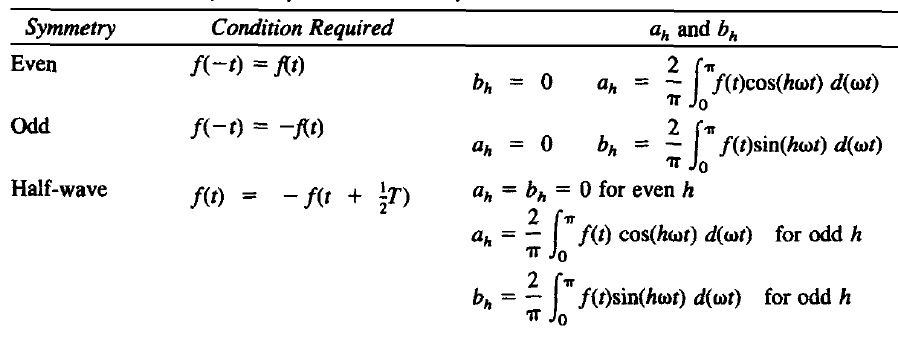
\includegraphics[width=2.5in,height=1in]{fouriert.png}
%	\caption{Fourier Transform Table}
%\end{figure}

% \begin{figure}[!ht]
% 	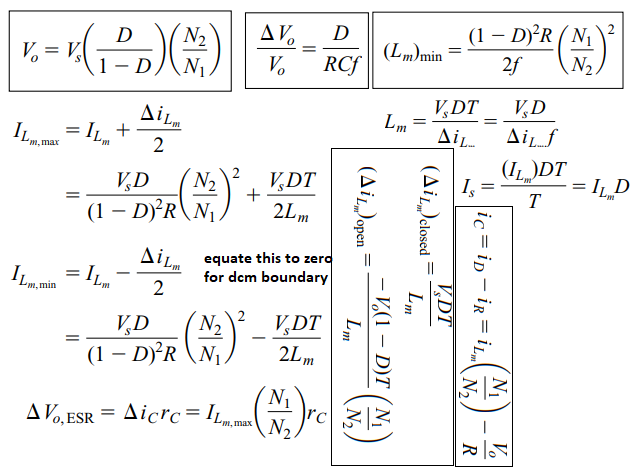
\includegraphics[width=3in,height=1.8in]{flybackformulasfromhart.png}
% 	\caption{Flyback Formulas}
% \end{figure}

% \begin{figure}[!ht]
% 	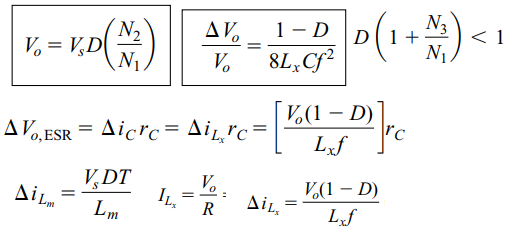
\includegraphics[width=3in,height=1.1in]{forwardsingleswitch.png}
% 	\caption{Forward (single switched) Converter Formulas}
% \end{figure}

% \begin{figure}[!ht]
% 	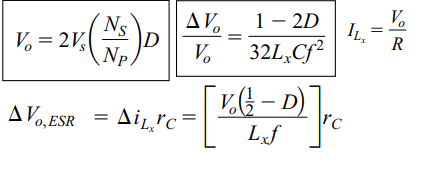
\includegraphics[width=3in,height=0.7in]{pushpull_someformulas.png}
% 	\caption{Push Pull Formulas}
% \end{figure}

\begin{figure}[!ht]
	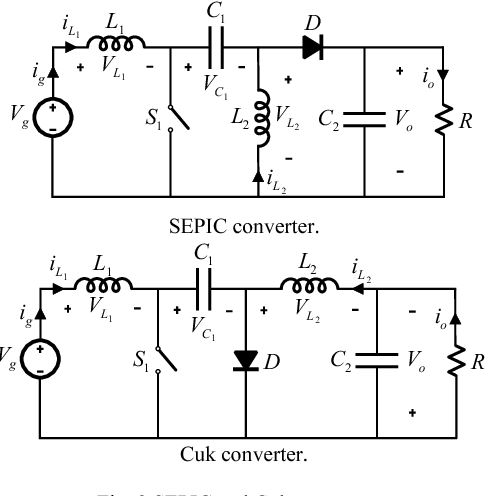
\includegraphics[width=2.5in,height=1.7in]{sepic_and_cuk_schematic.png}
	\caption{Sepic and Cuk Converter Schematics}
\end{figure}

\begin{figure}[!ht]
	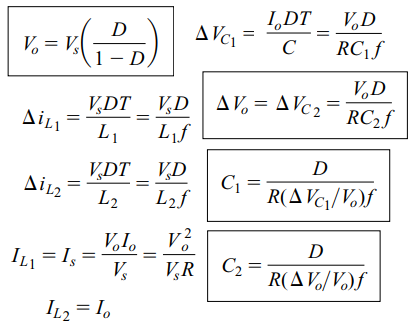
\includegraphics[width=2in,height=1.5in]{sepicformulas.png}
	\caption{Sepic Converter Formulas}
\end{figure}
\begin{figure}[!ht]
	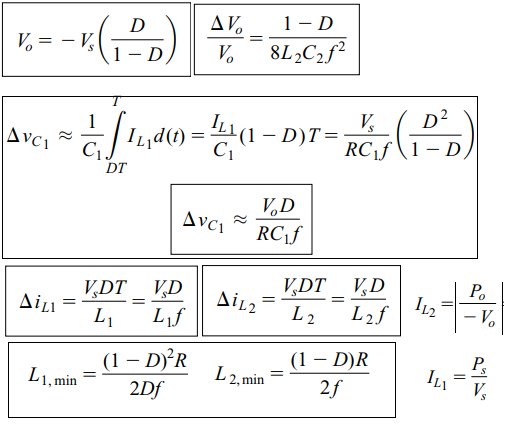
\includegraphics[width=2.2in,height=1.7in]{cukformulas.png}
	\caption{Cuk Converter Formulas}
\end{figure}

  \begin{figure}[!ht]
	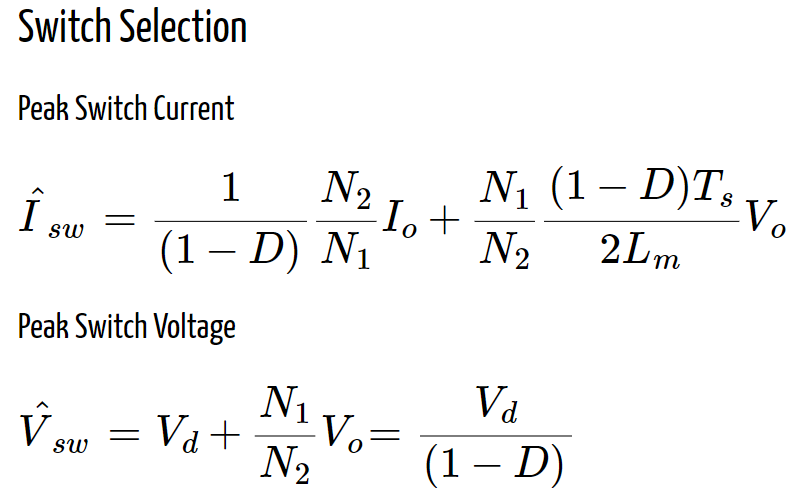
\includegraphics[width=2in,height=1in]{flybak_switch}
	\caption{Flyback switch considerations}
\end{figure}

\begin{figure}[!ht]
	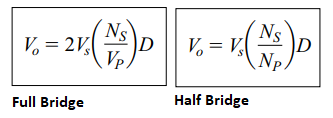
\includegraphics[width=1.6in,height=.6in]{fullandhalfinout.png}
	\caption{Full and Half Bridge Relations}
\end{figure}

\begin{figure}[!ht]
	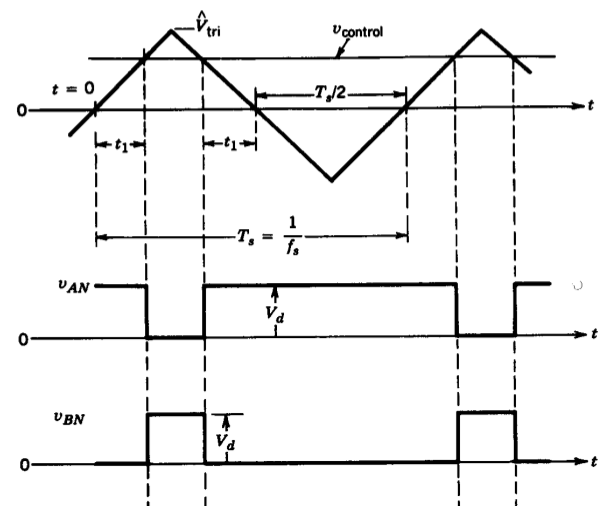
\includegraphics[width=2.5in,height=0.6in]{bipolar1.png}
	\caption{Bipolar Switching}
\end{figure}

\begin{figure}[!ht]
	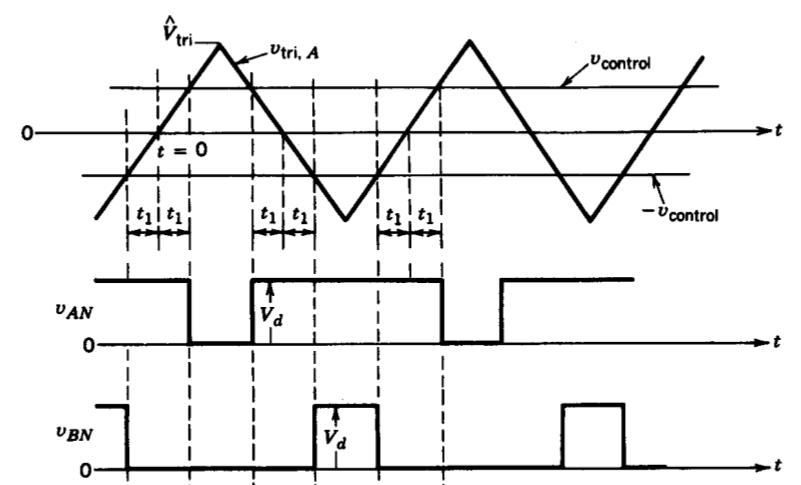
\includegraphics[width=2.5in,height=0.6in]{unipolar1.png}
	\caption{Unipolar switching}
\end{figure}

% \begin{equation}
% Switch Utilization= \frac{Po}{Psw}=\frac{Io.Vo}{q.Vswmax.Iswmax}
% \end{equation}

% $$ m_f=\dfrac{f_s}{f_1}, m_a=\dfrac{V_{control}}{V_{triangle}}$$
% $$m_a<1: linear, m_a>1: overmodulation$$

% \begin{figure}[!ht]
% 	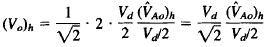
\includegraphics[width=2.3in,height=0.25in]{RmsVoltageofHarmonicsFullBridgeInverter.png}
% 	\caption{Rms Voltage of Harmonics Full Bridge Inverter}
% \end{figure}

%\begin{figure}[!ht]
%	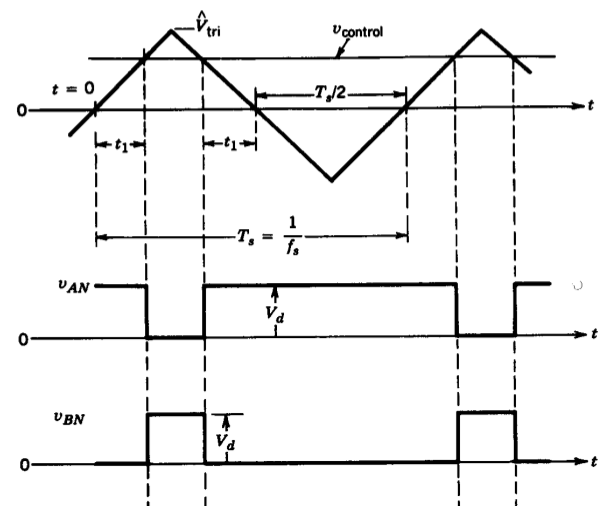
\includegraphics[width=2.5in,height=1in]{bipolar1.png}
%	\caption{Bipolar Switching}
%\end{figure}
%\begin{figure}[!ht]
%	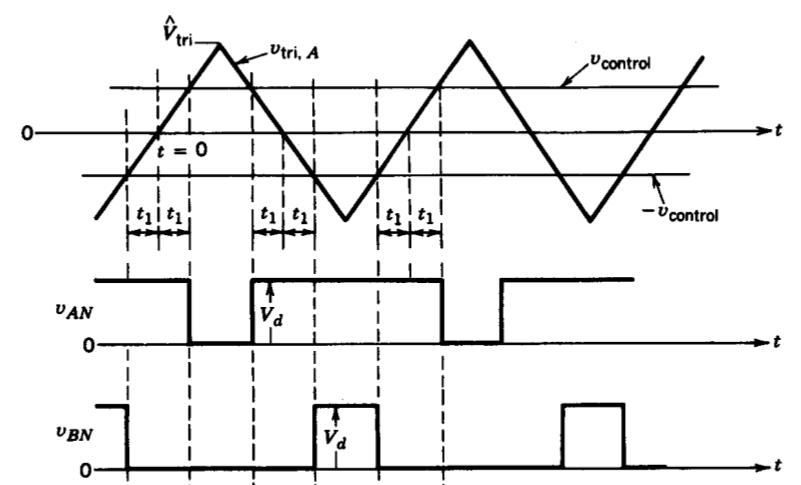
\includegraphics[width=2.5in,height=1in]{unipolar1.png}
%	\caption{Unipolar switching}
%\end{figure}

\subsection*{\small Cuk Converter}
\small
\begin{equation}
Vc1=Vo+Vd
\end{equation}

\begin{equation}
V_{rms}=\frac{2\pi}{\sqrt{2}}.N_{2}.f.B_{max}.A
\end{equation}



% Current Source Converter:
% \begin{equation}
% (V_o = V_d  (\dfrac{N_2}{N_1})(\dfrac{1}{2(1-D)})\\)
% \end{equation}




\subsection*{\small Signal Analysis}
 \begin{figure}[!ht]
	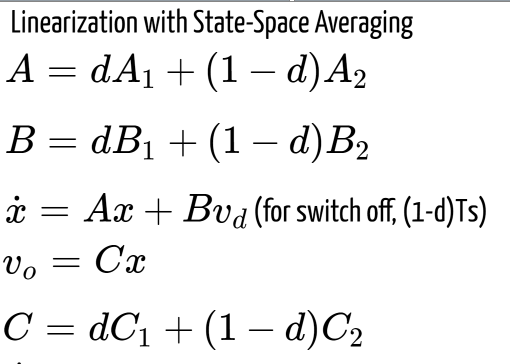
\includegraphics[scale=0.36]{ss1}
\hspace{0.05 cm}
	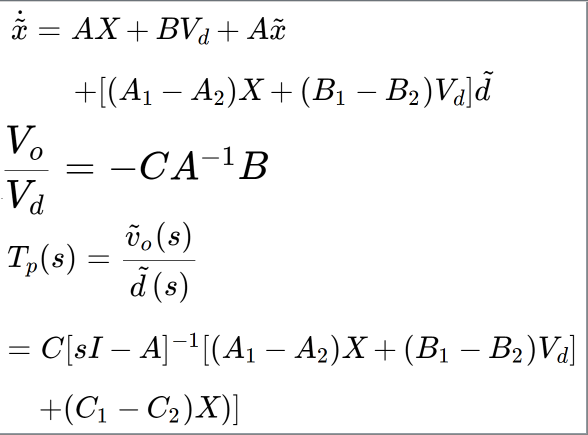
\includegraphics[scale=0.34]{ss2}
\end{figure}
\begin{equation*}
I_{o}=I_{lm}(1-D) 
\hspace{0.2cm}
I_{s}=I_{lm}(D)
\hspace{0.2cm}
At SS: AX+BV_{d}=0
\end{equation*}
For analysis, first derive generalstate space for on and off ccts, then decide which matrices are needed and which are 0. Cct analysis and derive matrices


\begin{table}[H]
\centering
\begin{tabular}{lllll}
    Topology & $V_{sw}$ & $I_{sw}$ & $V_{01,max}$ & q \\
    \hline

    Push Pull & $2V_{d,max}$ & $\sqrt2 \dfrac{I_{o,max}}{n}$ & $\dfrac{4}{\pi \sqrt2} \dfrac{V_{d,max}}{n}$ & 2 \\
    Half B. & $V_{d,max}$ & $\sqrt2 I_{o,max}$ & $\dfrac{4}{\pi \sqrt2} \dfrac{V_{d,max}}{2}$ & 2 \\
    Full B. & $V_{d,max}$ & $\sqrt2 I_{o,max}$ & $\dfrac{4}{\pi \sqrt2} V_{d,max}$ & 4 \\
 \end{tabular}   
  \caption{Swith Utilization doesnt change($1/2\pi$) for n:1 trans. ratio and in linear region scaled by $(m_{a}\pi)/4 $}
  
\end{table}



\end{document}
